\begin{frame}{Stratégies de simulation}{Équations d'ADR}
    \textbf{Stratégie $n^o1$ : Différencier le traitement sur chaque opérateur}\\
        Ne pas faire un schéma monolithique.
        \begin{itemize}
            \item Séparation d'opérateurs (\emph{splitting}) : $e^{\Delta t (A+B)} = e^{\frac{\Delta t}{2} A} \circ e^{\Delta t B} \circ e^{\frac{\Delta t}{2}A} + \mathcal{O}(\Delta t^2)$
            \item Méthodes ImEx (Additive Runge et Kutta) \cite{ASCHER1997151}
        \end{itemize}
        \pause
\noindent\color{Primary}\rule{\linewidth}{0.6pt}\color{black}

    \textbf{Stratégie $n^o2$ : Adaptation en espace par MRA} \cite{harten1994,Cohen2003}\\
        % --- image plein écran, uniquement sur l'overlay 2 ---
        \only<3>{
        \begin{tikzpicture}[remember picture,overlay]
            \node[inner sep=0] at (current page.center){
            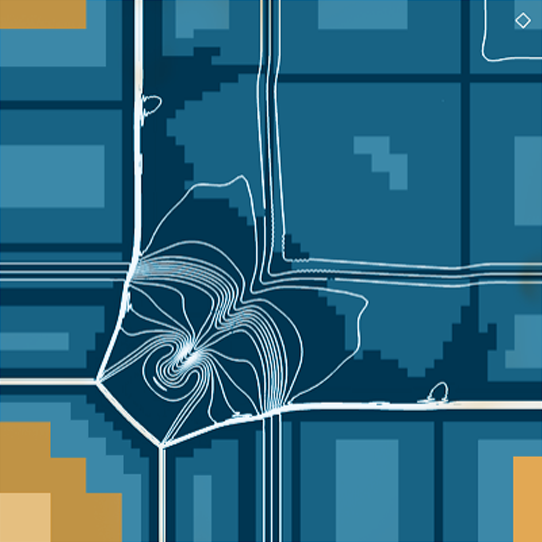
\includegraphics[height=\textheight]{medias/1_/exemple_compression_samurai.png}
            };
        \end{tikzpicture}
        }

        %%%     INSERER ICI 
\visible<4->{
\begin{itemize}
    \item Des grilles de \emph{résolution multiples},
    \item Deux opérateurs de \emph{projection/reconstruction},$\qquad$ \visible<7->{\color{Primary}{\textbf{Comment adapter ?}}} \color{black}
    \item Représentation de la solution comme une suite de \emph{détails},
    \item Une stratégie d'\emph{adaptation} : seuil de compression $\varepsilon$ et seuil local $\varepsilon_j = 2^{-j}\varepsilon$$\qquad$ \visible<8->{\color{Primary}{\textbf{\\Où adapter ?}}
      \begin{itemize}
        \item \color{black}{Baisse de la résolution : $\longrightarrow \cancel{d_k^j}$ si $d_k^j<\varepsilon_j$}
        \item \color{black}{Augmentation de la résolution : $d_k^{j-1}>2 \varepsilon_{j-1}$.}
      \end{itemize}}
\end{itemize}
}
\visible<4->{
\begin{tikzpicture}[>=Latex]
% ---- Styles de base
\tikzset{
  cell/.style={draw, thick, fill=gray!50},
  projHL/.style={}, % surbrillance projection (overlay 5)
  predHL/.style={}, % surbrillance prédiction (overlay 6)
  projHL_data/.style={fill=green!10}, % surbrillance projection (overlay 5)
  predHL_data/.style={fill=green!10}, % surbrillance projection (overlay 5)
  projArrow/.style={->, very thick},
  predArrow/.style={->, very thick, dashed}
}

% ---- Surbrillances dynamiques
\only<5>{\tikzset{projHL/.style={fill=red!10}}}     % slide 5 : projection
\only<6>{\tikzset{predHL/.style={fill=orange!10}}}     % slide 5 : projection


% ---- Légendes niveaux
\node[anchor=west] at (-8.5, -.25) {Niveau de résolution $j=3$};
\node[anchor=west] at (-8.5, .25)  {Niveau de résolution $j=2$};
\node[anchor=west] at (-8.5, .75)  {Niveau de résolution $j=1$};

% Axe x
\draw[->] (-4,-1) -- (4,-1);
\node[anchor=center] at (0, -1.23) {$x$};

% =======================
% NIVEAU j=1 (coarse)
% =======================
% Cellules (projection cible à droite, marquée pour overlay 5)
\draw[cell] (-4,.5) rectangle (0,1);
\draw[cell] (0,.5) rectangle (4,1); % <- cible projection (overlay 5)
\node at (-2, .75) {$u^1_0$};
\node at (+2, .75) {$u^1_1$};

% =======================
% NIVEAU j=2 (middle)
% =======================
% Cellules (prédiction source au milieu, marquée pour overlay 6)
\draw[cell,predHL_data] (-4,0) rectangle (-2,.5);
\draw[cell,predHL_data] (-2,0) rectangle (0,.5); % <- source prédiction (overlay 6)
\draw[cell,predHL_data] (0,0) rectangle (2,.5);  % <- contribue à projection (overlay 5)
\draw[cell,projHL] (2,0) rectangle (4,.5);  % <- contribue à projection (overlay 5)

\node at (-3, .25) {$u^2_0$};
\node at (-1, .25) {$u^2_1$};
\node at (+1, .25) {$u^2_2$};
\node at (+3, .25) {$u^2_3$};

% =======================
% NIVEAU j=3 (fine)
% =======================
% Cellules (sources projection à droite ; cible prédiction à gauche)
\draw[cell] (-4,-.5) rectangle (-3,0);
\draw[cell] (-3,-.5) rectangle (-2,0);
\draw[cell,predHL] (-2,-.5) rectangle (-1,0); % <- cellule prédite (overlay 6)
\draw[cell] (-1,-.5) rectangle (0,0);
\draw[cell] (0,-.5) rectangle (1,0);   % -> monte vers [0,0]--[2,.5]
\draw[cell] (1,-.5) rectangle (2,0);
\draw[cell,projHL_data] (2,-.5) rectangle (3,0);   % -> monte vers [2,0]--[4,.5]
\draw[cell,projHL_data] (3,-.5) rectangle (4,0);

\node at (-3.5, -.25) {$u^3_0$};
\node at (-2.5, -.25) {$u^3_1$};
\node at (-1.5, -.25) {$u^3_2$};
\node at (-0.5, -.25) {$u^3_3$};
\node at (+0.5, -.25) {$u^3_4$};
\node at (+1.5, -.25) {$u^3_5$};
\node at (+2.5, -.25) {$u^3_6$};
\node at (+3.5, -.25) {$u^3_7$};

% =======================
% FLÈCHES (dynamiques)
% =======================
% Slide 5 : PROJECTION (fine -> plus grossier)
\only<5>{
  % vers cellule [0,0]--[2,.5]
  % vers cellule [2,0]--[4,.5]
  \draw[projArrow,red] (2.5,-0.2) -- (2.85,0.25);
  \draw[projArrow,red] (3.5,-0.2) -- (3.15,0.25);

  % Légende
  \node[red,anchor=west] at (-3.8,-0.85) {\small Projection : agrégation fine $\rightarrow$ grossier};
}

% Slide 6 : PRÉDICTION (coarse -> plus fin)
\only<6>{
  % de [ -2,0 ]--[ 0,.5 ] vers [-2,-.5]--[-1,0]
  
  \draw[->,green,thick] (-1,0.25) -- (-1.25,-0.1);
  \draw[->,green,thick] (-2.5,0.25) -- (-1.5,-0.1);
  \draw[->,green,thick] (1,0.25) -- (-1.1,-0.2);
  

  % Légende
  \node[green!90!black,anchor=west] at (-3.8,-0.85) {\small Prédiction : interpolation grossier $\rightarrow$ fin};
}
\end{tikzpicture}}

\end{frame}